\chapter{Data} \label{Chap3}

\section{Dataset Overview}

The analytical dataset draws on five NWFP data sources: the site-wide meteorological station,
catchment soil moisture stations, eddy-covariance greenhouse-gas measurements, livestock-location
records, and field-event records. The greenhouse-gas source used here is the tower-based EC dataset.
A separate GreenFeed dataset measures emissions from individual animals but is excluded because it does
not represent the same tower-scale ecosystem exchange measured by EC. Table~\ref{tab:ch3_source_inventory}
summarises these sources, while detailed dictionaries describing downloaded raw variables and
project-derived variables are provided in Appendix~\ref{app:data-dictionary}.

{
\scriptsize
\setlength{\tabcolsep}{2pt}
\renewcommand{\arraystretch}{1.16}
\setlength\LTleft{0pt}
\setlength\LTright{0pt}
% \begin{longtable}{@{}p{0.22\textwidth}p{0.28\textwidth}p{\dimexpr0.50\textwidth-4\tabcolsep\relax}@{}}
\begin{longtable}{
@{}
>{\raggedright\arraybackslash}p{0.22\textwidth}
>{\raggedright\arraybackslash}p{0.28\textwidth}
>{\raggedright\arraybackslash}p{\dimexpr0.50\textwidth-4\tabcolsep\relax}
@{}
}
\caption{NWFP datasets used to construct the analytical dataset. Dataset scope follows the NWFP Data Guide and 
platform design guide \cite{hawkins2025,hawkins2023design}}
\label{tab:ch3_source_inventory}\\
\toprule
NWFP dataset & Availability and resolution & Contents \\
\midrule
\endfirsthead
\multicolumn{3}{l}{\tablename\ \thetable\ -- continued}\\
\toprule
NWFP dataset & Availability and resolution & Contents \\
\midrule
\endhead
\midrule
\multicolumn{3}{r}{Continued on next page}\\
\endfoot
\bottomrule
\endlastfoot
MET Station \cite{hawkins2023met} & 
31/10/2011--2 Mar 2026; 15 min & 
Site-level wind speed, air temperature, wind direction, relative humidity, solar radiation and precipitation \\

Soil Moisture Stations (SMS) \cite{hawkins2023sms} & 
31/10/2011--4 Mar 2024; 15 min & 
Catchment-level precipitation, soil moisture at 10 cm and soil temperature at 15 cm \\

Eddy Covariance Greenhouse Gas \cite{olde2023ec} & 
1/1/2017--1/1/2024; 30 min & 
Tower-level FCH\textsubscript{4}, FCO\textsubscript{2}, SSITC (quality) flags and associated EC biometeorological 
and turbulence variables, including VPD, PPFD, RN, USTAR and SHF \\

Livestock \cite{hawkins2025} & 
21/3/2011--21/4/2026; daily & 
Catchment-level daily location counts for livestock and weight \\

Field Events \cite{hawkins2023fieldevents} & 
5/1/2011--13/11/2025; event based, sparse & 
Field-level farm operations, grazing practices, silage, fertiliser additions \\
\end{longtable}
}

% Following time alignment and hourly aggregation, the consolidated table contained
% 70,153 hourly timestamps and 449 measurement variables. A modelling dataset with 30 
% variables for each tower from 2017 to 2025 is later constructed, 
% with valid coverage for EC modelling from 2017 to 1 January 2024. However, valid
% FCH\textsubscript{4} coverage within that window is not uniform across towers, 
% as will be discussed in the next section.

Following time alignment and hourly aggregation, the consolidated table
contained 70,153 hourly timestamps and 449 measurement variables. The hourly
gap-filling frame later uses 30 predictors per tower, while forecasting uses
the separate daily predictor frame described in Chapter~\ref{Chap5}. EC target
analysis is restricted to the period from 1 January 2017 to 1 January 2024.

% ############################################################################
\section{Exploratory Data Analysis and Data Preparation}
% ############################################################################
\subsection{Methane Target Availability}

Target availability was assessed over the common 61,344-hour EC analysis window from 1 January
2017 to 1 January 2024. Raw missingness indicates whether an hourly FCH\textsubscript{4} value is
present in the consolidated data. The modelling target is stricter: an observation is usable only
when its SSITC quality class is 0 or 1 and its flux lies within the project plausibility range of
$[-500,3000]$ nmol m$^{-2}$ s$^{-1}$. Table~\ref{tab:ch3_fch4_missingness} distinguishes these two
stages, while Figure~\ref{fig:ch3_fch4_availability} shows both the temporal behaviour of the usable
target and its annual completeness.

\begin{table}[htbp]
\centering
\small
\caption{Availability of hourly FCH\textsubscript{4} observations over the common 2017--2023 EC
analysis window. QC-valid observations pass the SSITC and plausibility filters used to construct the
modelling target.}
\label{tab:ch3_fch4_missingness}
\begin{tabular*}{\textwidth}{@{\extracolsep{\fill}}lrrrr@{}}
\toprule
Tower & Raw observed (h) & Raw missing (\%) & QC-valid (h) & Unavailable after QC (\%) \\
\midrule
T2 & 8,099 & 86.8 & 4,890 & 92.0 \\
T4 & 30,485 & 50.3 & 19,469 & 68.3 \\
T9 & 17,509 & 71.5 & 11,235 & 81.7 \\
\bottomrule
\end{tabular*}
\end{table}

\begin{figure}[htbp]
\centering
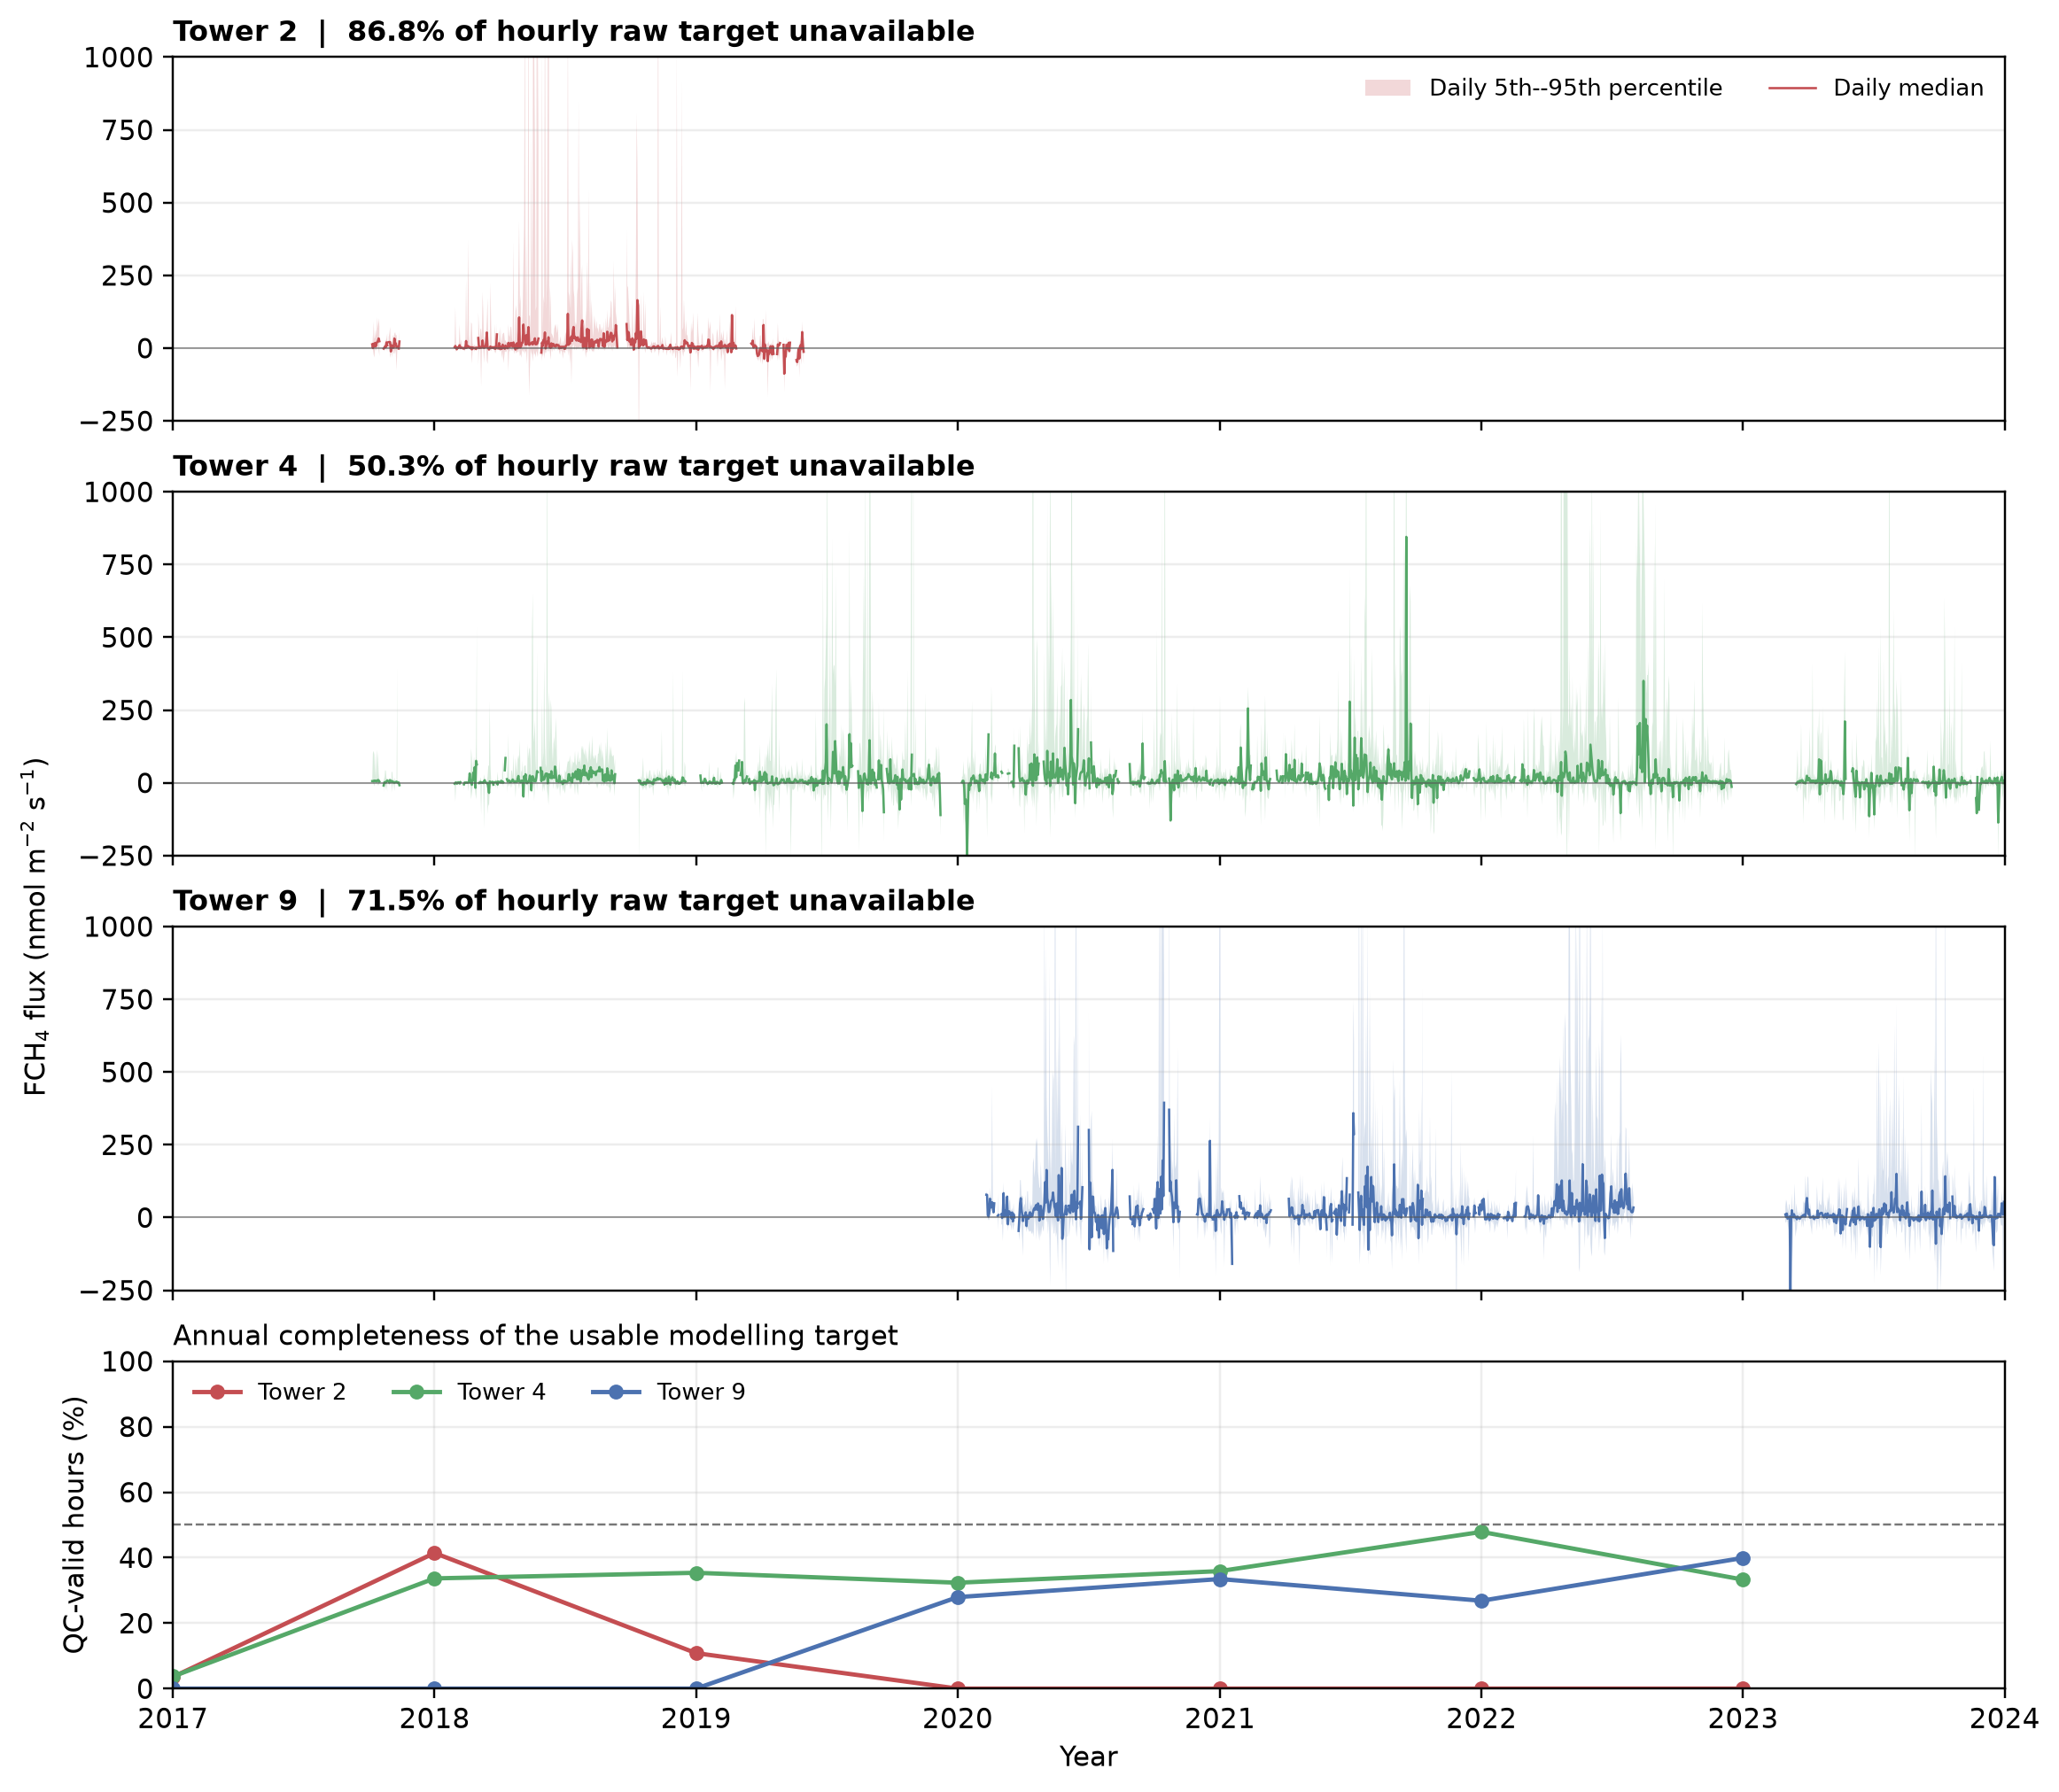
\includegraphics[width=\textwidth]{Figures/ch3_fch4_three_tower_availability.png}
\caption{
    Daily median FCH\textsubscript{4} flux (line) and 5th--95th percentile range (shaded) at towers T2, 
    T4, and T9, with hourly raw-data unavailability noted per panel. Bottom panel: annual 
    completeness of the QC-valid modelling target. Note that y-axis has been limited to $[-250,1000]$ 
    nmol m$^{-2}$ s$^{-1}$ for readability.
}
\label{fig:ch3_fch4_availability}
\end{figure}


Methane-target coverage is limited across all towers, with 92.0\% of common-window hours unavailable at T2, 
compared with 68.3\% at T4 and 81.7\% at T9. Missingness is temporally structured: T2 observations are 
concentrated in 2017--2019, after which its methane analyser was relocated to T9 following the Red 
farmlet's conversion to arable production \cite{olde2023ec}. T2 results should be interpreted cautiously due to its smaller, temporally 
narrower sample.

\FloatBarrier

% ############################################################################
\subsection{Quality Control and Environmental Variable Gap-Filling}
\label{sec:ch3_environmental_preparation}

Quality screening was applied before reconstruction so that rejected observations could not act as
anchors for filling. Hourly FCH\textsubscript{4} and FCO\textsubscript{2} observations were retained
only when their SSITC class was 0 or 1; values outside $[-500,3000]$~nmol
CH\textsubscript{4}~m$^{-2}$~s$^{-1}$ and $[-100,100]$~$\mu$mol
CO\textsubscript{2}~m$^{-2}$~s$^{-1}$, respectively, were set to missing. The effect on the methane
target is reported in Table~\ref{tab:ch3_fch4_missingness}. Before environmental-driver filling,
friction velocity was restricted to $[0,3]$~m~s$^{-1}$ and vapour-pressure deficit to $[0,15]$ on
the stored numerical scale because both fields contained extreme values. A separate low-turbulence
flag was retained as a diagnostic rather than used to reject FCH\textsubscript{4}, since such
filtering is not assumed to be a generally valid methane quality criterion.

Environmental-driver preparation combined two related procedures. The auxiliary-data calibration
workflow, detailed in Algorithm~\ref{alg:auxiliary-driver-gapfill} in
Appendix~\ref{app:data-dictionary}, was adapted from the North Wyke Farm Platform EC processing
report \cite{nwfp2022ecqc}. The subsequent temporal filling hierarchy was
implemented in Python and informed by the interpolation and mean-diurnal-course principles provided
by \texttt{REddyProc} \cite{wutzler2018reddyproc}; the R package itself was not invoked. The active
data path used the central MET station for shortwave radiation, air temperature and wind speed, the
corresponding catchment SMS for precipitation and soil conditions, and EC records for VPD, PPFD, net
radiation, friction velocity and soil heat flux.

Following source selection and plausibility screening, internal gaps were linearly interpolated for
up to 288 hours for air temperature, VPD, wind speed, soil moisture and soil temperature, and for up
to two hours for the remaining drivers. Unresolved gaps were filled from the mean diurnal course at
the same hour of day, first within a centred seven-day window and then, where necessary, within 14-,
28- and 60-day windows. Remaining gaps received the corresponding hour-of-day median and, only when
that was unavailable, the series-wide median. Accepted observations were preserved throughout the
temporal filling sequence. The resulting drivers are numerically complete while retaining local
diurnal structure where nearby observations exist; values produced during longer sensor blackouts
remain reconstructions rather than new measurements. This preprocessing was applied only to supporting 
model inputs; observed FCH\textsubscript{4} values were not imputed.

\begin{table}[htbp]
\centering
\small
\caption{
    Prior availability and synthetic-gap reconstruction accuracy of environmental drivers.
    Gap-CV $R^2$ is the mean across towers of the tower-level median over five gap-duration 
    (1h, 4h, 32h, 288h, mixed) scenarios. Each scenario masks 25\% of eligible observations 
    across two repetitions for evaluation. The auxiliary-data calibration component is detailed in
    Algorithm~\ref{alg:auxiliary-driver-gapfill} in Appendix~\ref{app:data-dictionary}.
}
\label{tab:ch3_environmental_gapfill}
\begin{tabular*}{\textwidth}{@{\extracolsep{\fill}}lrrrrr@{}}
\toprule
& \multicolumn{3}{c}{Available input (\%)} & \multicolumn{1}{c}{After filling (\%)}
& \multicolumn{1}{c}{Gap-CV $R^2$} \\
\cmidrule(lr){2-4}\cmidrule(lr){5-5}\cmidrule(l){6-6}
Driver & T2 & T4 & T9 & All towers & Mean across towers \\
\midrule
Shortwave radiation & 98.8 & 98.8 & 98.8 & 100.0 & 0.685 \\
Air temperature & 98.8 & 98.8 & 98.8 & 100.0 & 0.692 \\
Vapour-pressure deficit & 61.8 & 75.4 & 73.2 & 100.0 & 0.471 \\
Photosynthetic photon flux & 61.1 & 86.2 & 81.8 & 100.0 & 0.695 \\
Net radiation & 60.2 & 86.2 & 81.8 & 100.0 & 0.738 \\
Wind speed & 93.6 & 93.6 & 93.6 & 100.0 & 0.482 \\
Friction velocity & 81.2 & 88.2 & 84.4 & 100.0 & 0.000 \\
Soil heat flux & 43.3 & 86.2 & 81.8 & 100.0 & 0.532 \\
Precipitation & 83.1 & 85.7 & 62.5 & 100.0 & 0.012 \\
Soil moisture & 81.1 & 64.6 & 75.5 & 100.0 & 0.997 \\
Soil temperature & 83.7 & 65.6 & 78.9 & 100.0 & 0.993 \\
FCO\textsubscript{2} & 50.5 & 64.2 & 58.5 & 100.0 & 0.745 \\
\bottomrule
\end{tabular*}
\end{table}

Mean driver availability before reconstruction was 77.0\% at T2, 84.5\% at T4, and 82.8\% at T9. 
The staged procedure achieved 100\% numerical coverage across all 33 tower--driver series, but 
reconstruction accuracy varied considerably. Gap-CV performance was strongest for soil moisture and 
temperature, while precipitation and friction velocity showed limited skill. Thus, complete coverage 
does not imply equally reliable reconstruction across drivers. Their downstream contributions are 
evaluated in Chapter~\ref{Chap4}.

% ############################################################################
\subsection{Temporal Analysis and Dimensionality Reduction}

ACF and PACF were used to examine temporal dependence in the QC-valid
observed FCH\textsubscript{4} series without reconstructing long target
gaps. Weekly STL decomposition was also applied to the longest
sufficiently complete daily segment at each tower. Full diagnostics are
provided in Appendix Figures~\ref{fig:appendix_ch3_acf_pacf} and
\ref{fig:appendix_ch3_stl}.

Pairwise associations with the target were calculated from the same 30-predictor frame used in
the gap-filling experiments. Tower indicators were excluded because they are constant within each
tower, and correlations were calculated only where observed FCH\textsubscript{4} passed the target
quality and plausibility filters; gap-filled FCH\textsubscript{4} values were not used. Spearman's
rank correlation was selected because the target is highly skewed and spike-dominated, making a
rank-based measure more representative of monotonic association than Pearson correlation. The
calculation was performed separately for each tower using pairwise-complete observations.
For a concise comparison, Figure~\ref{fig:ch3_target_correlations} takes the five largest absolute
correlations within each tower and displays their union, while retaining all three tower coefficients
for every selected predictor. The complete 30-predictor matrix is provided in
Appendix Figure~\ref{fig:appendix_target_correlations_full}.

\begin{figure}[htbp]
\centering
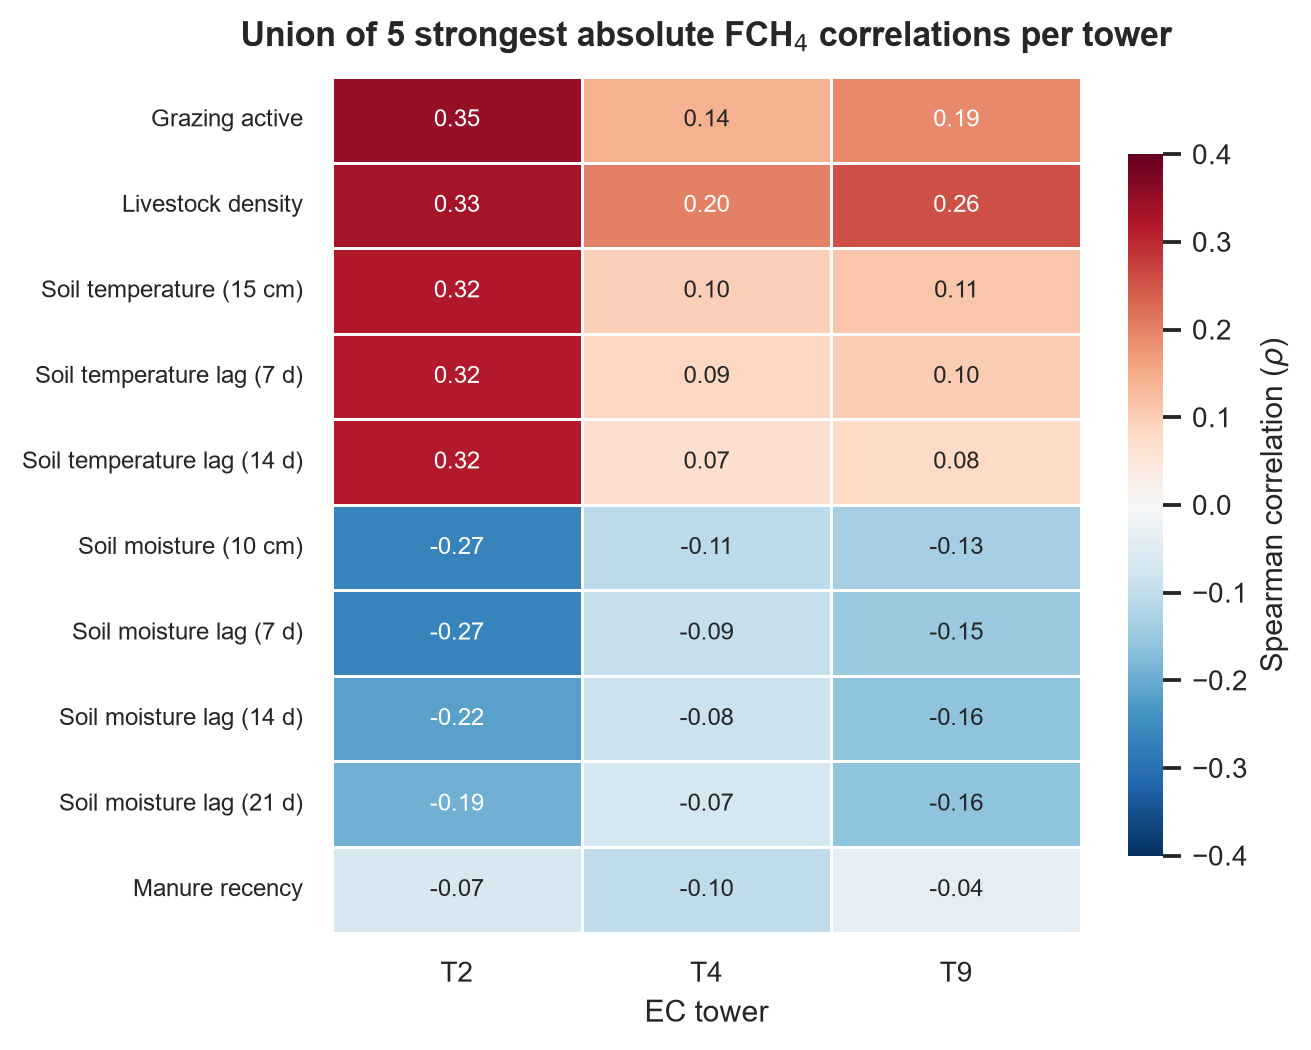
\includegraphics[width=0.82\textwidth]{Figures/ch3_fch4_target_correlations.png}
\caption{Strongest Spearman associations between observed QC-valid FCH\textsubscript{4} and the
gap-filling predictors. The displayed variables are the union of the five largest absolute
correlations selected independently within each EC tower; coefficients for all three towers are
then shown for every selected variable. Positive values indicate that larger predictor values tend
to accompany larger methane fluxes, whereas negative values indicate an inverse monotonic
association.}
\label{fig:ch3_target_correlations}
\end{figure}

Figure~\ref{fig:ch3_target_correlations} shows that livestock density has the strongest consistent
positive association across the three towers ($\rho=0.33$, $0.20$, and $0.26$ at T2, T4, and T9,
respectively), with grazing status showing the same direction. Soil moisture and its lagged values
are generally negatively associated with FCH\textsubscript{4}, whereas soil temperature is
positively associated, particularly at T2. However, all absolute correlations remain below 0.35
and their magnitudes differ substantially by tower. These coefficients therefore provide an
initial screening of the feature space rather than a feature-importance result: they do not capture
nonlinear interactions, and the closely related soil-lag variables share overlapping information.

Multivariate structure was examined using the same 11 environmental drivers employed by the
gap-filling pipeline. TICA \cite{perezhernandez2013} was fitted at a 24-hour lag after standardisation, 
treating each tower as a separate contiguous trajectory so that lagged pairs could not cross tower or deployment
boundaries. UMAP \cite{mcinnes2018umap} was fitted to a tower-balanced sample of 3,000 hours using 30 neighbours and a
minimum distance of 0.15. Neither analysis used FCH\textsubscript{4}, tower indicators, deterministic
calendar encodings or precomputed lag features as inputs; methane availability was introduced only
after fitting as a visual label. 

\begin{figure}[htbp]
\centering
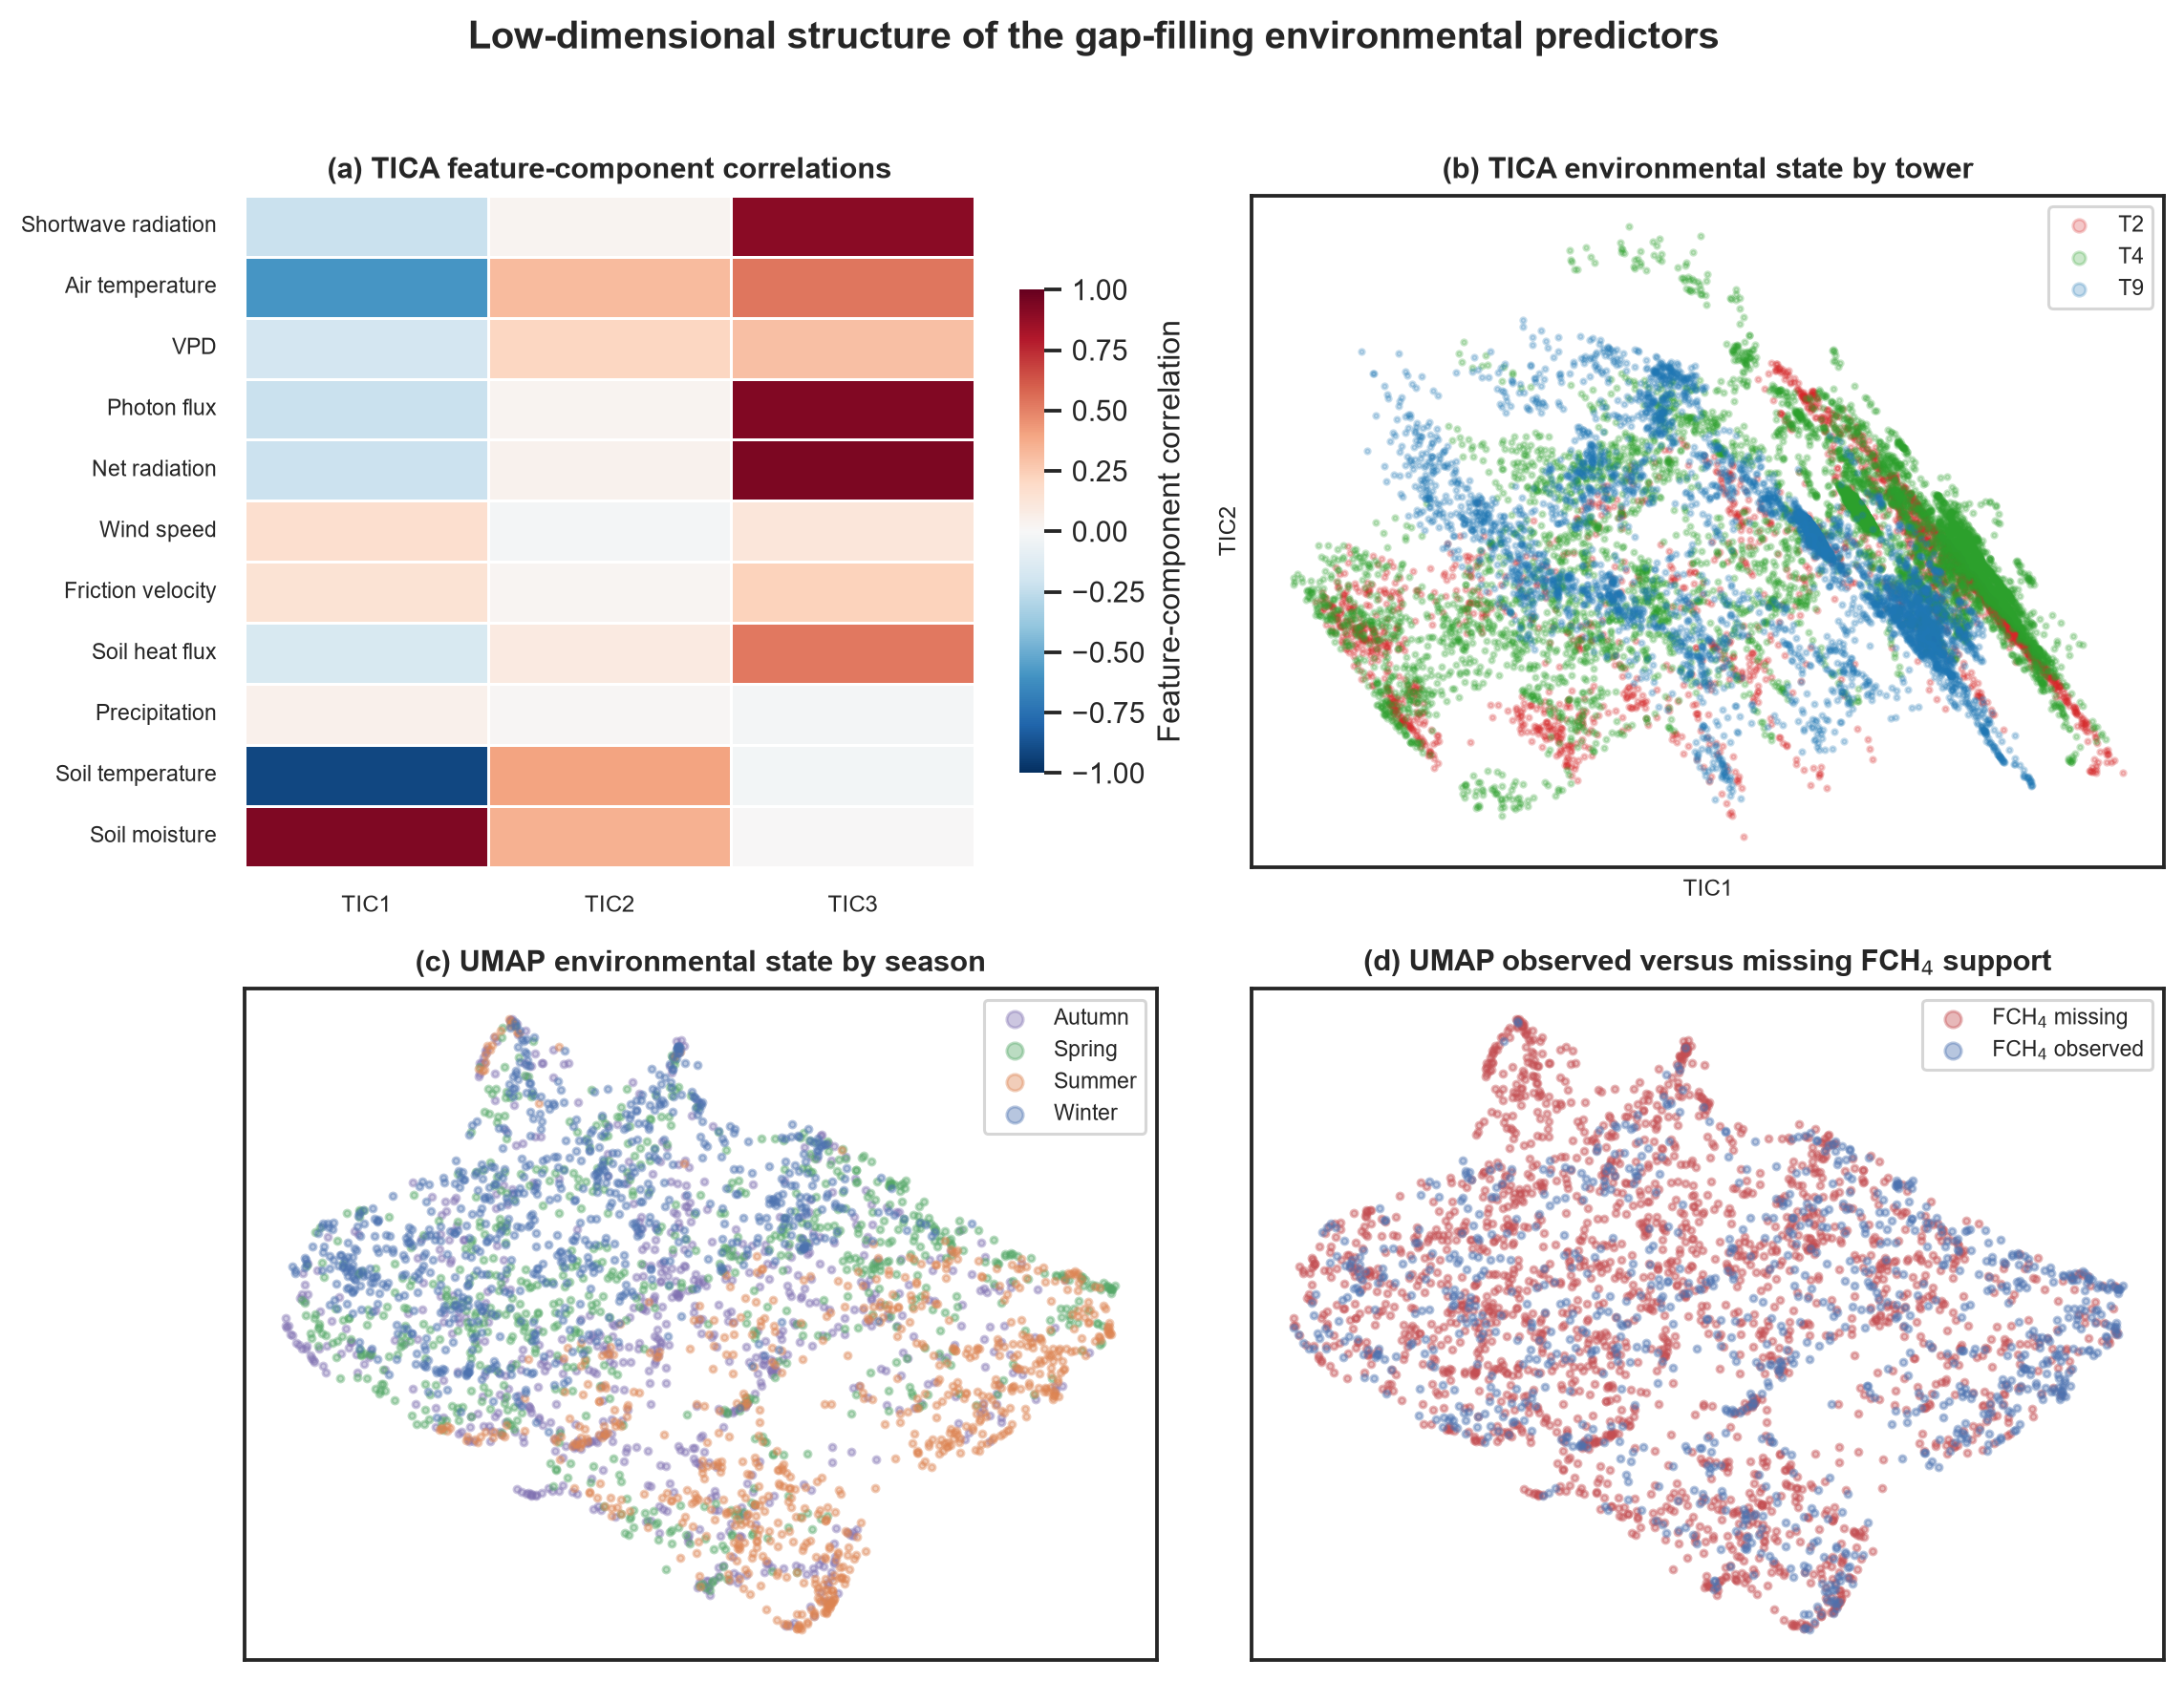
\includegraphics[width=\textwidth]{Figures/ch3_tica_umap_embeddings.png}
\caption{Low-dimensional structure of the environmental predictors used by the gap-filling
pipeline. Panel (a) shows feature--component correlations for three TICA components at a 24-hour
lag; panel (b) shows the first two TICA components by EC tower. Panels (c) and (d) show the same
saved UMAP embedding coloured by season and by observed versus missing FCH\textsubscript{4},
respectively. }
\label{fig:ch3_tica_umap}
\end{figure}

At a 24-hour lag, the first three TICA components had autocorrelations of 0.992, 0.970 and 0.869, 
implying timescales of 122, 33 and 7 days. The slowest component correlated 
strongly with soil moisture (0.93), soil temperature (0.91) and air temperature (0.59). UMAP showed 
moderate clustering by tower and season, but little separation between observed and missing FCH\textsubscript{4} 
hours. The two groups therefore occupy overlapping environmental space, though this does 
not establish that target missingness is random.

These diagnostics informed the final predictor design, but their
low-dimensional representations were not retained. The observed temporal
dependence supports the use of multi-scale lagged and rolling environmental
variables, while fold-safe experiments found no consistent improvement from
adding TICA components or UMAP-informed neighbour features. The final
gap-filling and forecasting models therefore use the original environmental
variables.
